%% ============================================================
%% TRIsecure: South African Computer Journal (SACJ) Submission
%%
%% HOW TO COMPILE ON OVERLEAF:
%%   1. Download sacjsub.cls from the SACJ submissions page:
%%      https://journals.assaf.org.za/index.php/sacj/about/submissions
%%      (look for "Complete LaTeX example")
%%   2. Upload sacjsub.cls to this Overleaf project
%%   3. Copy all PNG files from springer/figures/ into the
%%      figures/ subfolder here
%%   4. Set Compiler = pdfLaTeX, Bibliography = BibTeX
%%   5. Compile: pdfLaTeX -> BibTeX -> pdfLaTeX -> pdfLaTeX
%%
%% DOUBLE-BLIND REVIEW (SACJ policy):
%%   Author names do NOT appear in the PDF for review.
%%   \SACJauthor and \SACJaddress lines are commented out.
%%   Enter all author details via the journal web form at submission.
%%   Uncomment those lines ONLY after acceptance for the final version.
%%
%% FIGURES NOTE:
%%   SACJ prefers PDF/EPS vector or TIFF (600 dpi). PNG is accepted
%%   as a last resort. Convert figures for the final accepted version.
%% ============================================================

\documentclass[submission]{sacjsub}

%% -- Packages not included in sacjsub by default -------------
\usepackage[T1]{fontenc}
\usepackage[utf8]{inputenc}
\usepackage{amsmath,amssymb}
\usepackage{graphicx}
\usepackage{booktabs}
\usepackage{multirow}
\usepackage{tabularx}
\usepackage{algorithm}
\usepackage{algorithmicx}
\usepackage{algpseudocode}
\usepackage[shortlabels]{enumitem}
\usepackage{url}
\usepackage[expansion=false]{microtype}

%% -- Theorem environment -------------------------------------
\newtheorem{theorem}{Theorem}

%% -- tabularx ragged-right column type -----------------------
\newcolumntype{R}{>{\raggedright\arraybackslash}X}

%% =============================================================
\begin{document}
%% =============================================================

%% --- Title --------------------------------------------------
%% SACJ: title should be as brief as possible
\SACJtitle{TRIsecure: Design and Evaluation of a Three-Factor
  Post-Quantum Biometric E-Voting Framework on Commodity Edge Hardware}

%% --- Authors ------------------------------------------------
%% BLIND SUBMISSION: author block withheld for peer review.
%% Uncomment below ONLY after acceptance for the camera-ready version.
%%
%% \SACJauthor[a]{Pinnemcharla Sai Vivek Reddy}{ch.sc.u4cys23034@ch.students.amrita.edu}{}
%% \SACJauthor[a]{Saranya G}{g\_saranya@ch.amrita.edu}{corresponding}
%% \SACJauthor[a]{S.\ Udhaya Kumar}{u\_udhayakumar@ch.amrita.edu}{}
%% \SACJaddress[a]{Department of Computer Science and Engineering,
%%   Amrita Vishwa Vidyapeetham, Chennai, Tamil Nadu, India}

%% --- Running header ------------------------------------------
\SACJrunningheader{[Blind review]}{TRIsecure: PQ Biometric E-Voting}

%% --- Citation authors (foot of title page) ------------------
%% For camera-ready, replace the line below with the real author list:
%% \SACJcitationauthors{Pinnemcharla Sai Vivek Reddy, Saranya G and S.\ Udhaya Kumar (year).}
\SACJcitationauthors{[Authors omitted for blind review]}

%% --- Abstract -----------------------------------------------
%% SACJ requirement: FEWER THAN 200 WORDS.
%% No references, footnotes, or special symbols in the abstract.
\SACJabstract{Electronic voting systems must jointly satisfy voter
authentication, vote integrity, end-to-end verifiability, and
practical deployment on resource-limited hardware, requirements that
existing systems treat in isolation. TRIsecure V2 is a three-factor
biometric e-voting terminal that satisfies all four requirements on a
commodity Raspberry Pi 4 without server-grade infrastructure or cloud
connectivity. The system integrates ISO/IEC 19795-1 compliant Bayesian
fusion of face recognition and NFC card modalities, ISO/IEC 30107-3
presentation attack detection, a hybrid post-quantum cryptographic
layer per NIST FIPS 203/204, and a formally verified five-stage
authentication protocol with six proved security properties. A novel
Adaptive Trust Score engine dynamically adjusts component weights based
on contextual risk signals, routing borderline cases for supervisor
review rather than binary rejection. Simulation-based evaluation
achieves EER of 1.55 percent, AUC of 0.9991, and ACER of 4.25
percent. A pilot study with 20 participants on real hardware confirms
zero error rates across 271 authentication events. On-device
benchmarking delivers 110.7 ms end-to-end authentication latency and
541.6 voters per minute throughput. To our knowledge, no prior
e-voting system simultaneously provides formal protocol verification,
post-quantum cryptography, adaptive trust scoring, liveness detection,
and end-to-end verifiability on low-cost edge hardware.}

%% --- ACM Computing Classification System 2012 ---------------
%% Use the 2012 CCS only: https://dl.acm.org/ccs/ccs.cfm
%% The 1998 system is NOT accepted by SACJ.
%% Third argument: h = highly relevant, m = moderately, l = low
\SACJACMCategory{Security and privacy}{Authentication}{h}
\SACJACMCategory{Security and privacy}{Cryptography}{m}
\SACJACMCategory{Applied computing}{Computers in other domains}{m}

%% --- Keywords -----------------------------------------------
\SACJkeywords{biometric authentication, e-voting, post-quantum
cryptography, formal verification, edge computing, presentation attack
detection, Bayesian fusion, Merkle proof, NFC authentication, adaptive
trust scoring}

%% --- Generate the title block -------------------------------
\SACJmaketitle

%% =============================================================
\section{Introduction}\label{sec:intro}

Electronic voting systems are critical infrastructure where failure
consequences are asymmetric: a single undetected fraud vector can
undermine election legitimacy at scale. The fundamental security
challenge is to authenticate the right voter, record the right vote,
prevent tampering, and allow the voter to verify their
participation---all while running on deployable, affordable hardware.

Existing systems leave at least one requirement unsatisfied.
Fingerprint- and face-based voting
systems~\cite{bello2021biometric,sanchez2020biometric,komatineni2020biometric,nagaraj2022voting}
report biometric error rates without formal protocol verification or
post-quantum (PQC) readiness. Blockchain-based
approaches~\cite{ayed2017conceptual,hardwick2018voting,faruk2024transforming}
provide strong vote integrity but lack biometric authentication and
rely on classical cryptography vulnerable to quantum
adversaries~\cite{bernstein2017post}; a comprehensive review of 81
blockchain voting systems by Huang et al.~\cite{huang2022blockchain_voting}
confirms this gap. Industry multi-factor authentication standards
(FIDO2/WebAuthn~\cite{fido2_webauthn}) are not designed for the
one-time-per-election voting constraint and do not incorporate formal
liveness detection or voter-verifiable receipts.

To the best of our knowledge, no existing e-voting system jointly
provides: (i)~multi-factor biometric authentication with liveness
detection, (ii)~formally verified protocol security, (iii)~post-quantum
cryptographic readiness, and (iv)~end-to-end voter
verifiability---all on low-cost edge hardware without requiring cloud
connectivity.

\subsection*{Contributions}

We address these gaps with \textbf{TRIsecure V2}:

\begin{enumerate}[label=\textbf{C\arabic*.},leftmargin=*]
  \item \textbf{Formally verified authentication.} A five-stage
        pipeline modelled as a DFA with six proved security properties:
        determinism, completeness, safety, liveness, double-vote
        prevention, and rate-limit enforcement.
  \item \textbf{Bayesian biometric fusion.} Log-likelihood-ratio
        fusion of face cosine similarity and NFC channel evidence
        (EER\(=1.55\%\), AUC\(=0.9991\), TAR@1\%FAR\(=97.7\%\)).
  \item \textbf{Hybrid post-quantum layer.} Kyber-768\(+\)X25519 KEM
        (FIPS~203) and Dilithium-3\(+\)Ed25519 signatures (FIPS~204);
        ML-KEM-768 encaps 0.088~ms, ML-DSA-65 sign 1.536~ms on-device.
  \item \textbf{ISO/IEC~30107-3 PAD.} MiniFASNetV2 liveness
        detection (BPCER\(=1.0\%\), ACER\(=4.25\%\)).
  \item \textbf{End-to-end verifiability.} SHA-256 receipts and
        \(O(\log n)\) Merkle inclusion proofs.
  \item \textbf{Edge evaluation.} Raspberry Pi~4 (ARM64, 4~GB):
        110.7~ms latency (p99\(=111.3\)~ms), 541.6~voters/min.
  \item \textbf{Adaptive Trust Score (ATS) engine.} A context-aware
        weighted fusion model that adjusts face/NFC/PAD component
        weights dynamically based on risk signals, producing
        HIGH/MEDIUM/LOW trust decisions. Genuine users achieve 99.3\%
        HIGH trust; 100\% of simulated impostor attempts are rejected.
  \item \textbf{Adversarial attack evaluation.} Six attack categories
        quantify per-layer defence contribution; the full defence stack
        reduces combined success from \(\approx35\%\) to zero simulated
        bypass events after NFC-AES-GCM.
  \item \textbf{Proof-of-concept hardware pilot.} End-to-end
        validation with \(N{=}20\) participants across 271
        authentication events: FAR\(=\)FRR\(=\)ACER\(=0.00\%\).
\end{enumerate}

The \textbf{novel contributions} are: (i)~the ATS engine, which
introduces dynamic risk-adaptive weight adjustment absent from all prior
biometric e-voting systems; (ii)~their \emph{principled co-design}; and
(iii)~the \emph{complete systems security architecture}---a fully
deployable secure voting terminal on low-cost edge hardware. To the best
of our knowledge, no prior e-voting system delivers all six security
properties simultaneously on a Raspberry Pi class device.

%% =============================================================
\section{Related Work}\label{sec:related}

\subsection{Biometric E-Voting Systems}

Bello et al.~\cite{bello2021biometric} achieve EER~\(=2.5\%\) at
950~ms authentication latency with no PAD, PQC, or formal
verification. S\'{a}nchez-Reillo et al.~\cite{sanchez2020biometric}
report EER~\(=3.2\%\) at 480~ms on constrained hardware. Komatineni
and Lingala~\cite{komatineni2020biometric} combine machine-learning
face detection with biometric scanning for duplicate-vote prevention.
Nagaraj et al.~\cite{nagaraj2022voting} integrate facial recognition
with fingerprint authentication to strengthen polling station security.
Megalingam et al.~\cite{megalingam2022voter} combine a voter
identification card with fingerprint biometrics achieving low-cost
deployment, but provide no liveness detection, formal protocol
verification, or post-quantum cryptography. Varma and
Megalingam~\cite{varma2025fpga} demonstrate FPGA-accelerated biometric
voting but lack PQC support and verifiable receipts. Revathy et
al.~\cite{revathy2022cnn_evoting} integrate CNN-based face recognition
with blockchain and blind signatures. Faruk et
al.~\cite{faruk2024transforming} deploy blockchain and biometric
verification over Hyperledger Fabric, demonstrating 87\% biometric
registration success across 100 participants but relying on classical
cryptography. George et al.~\cite{george2024adaptive_biometric}
demonstrate EdgeFace, a compact model achieving sub-1\% EER on mobile
ARM, confirming the feasibility trajectory of high-accuracy face
recognition on the same hardware class as TRIsecure~V2. Buchmann et
al.~\cite{buchmann2024pvoting} provide a 2024 systematic review of
remote e-voting security, identifying formal verification and biometric
binding as the two most significant unresolved gaps across all deployed
systems.

\subsection{Blockchain-Based Voting}

Fujioka et al.~\cite{fujioka1992practical} proposed the foundational
blind-signature-based secret ballot scheme; Benaloh and
Tuinstra~\cite{benaloh1994receipt} formalised receipt-freeness.
Ayed~\cite{ayed2017conceptual} proposes Ethereum-based voting
(\(>2{,}100\)~ms) with PIN-only authentication. Hardwick et
al.~\cite{hardwick2018voting} and Hj\'{a}lmarsson et
al.~\cite{hjalmarsson2018blockchain} extend this with anonymisation,
but provide no biometric gate or anti-spoofing. Durga et
al.~\cite{durga2022blockchain} propose a private blockchain mechanism
for online voting but rely on classical cryptography with no biometric
identity binding. Huang et al.~\cite{huang2022blockchain_voting} survey
blockchain applications in voting across 81 prior works (ACM Computing
Surveys 2022), identifying voter authentication and anti-spoofing as
the primary unresolved gaps. TRIsecure~V2 achieves equivalent vote
integrity via hash chaining and Merkle proofs without blockchain
overhead, while adding biometric authentication.

\subsection{Post-Quantum Cryptography on Edge}

Sikeridis et al.~\cite{sikeridis2020pqc} show Kyber-768 and
Dilithium-3 are feasible in TLS~1.3 on ARM devices via liboqs. Paquin
et al.~\cite{paquin2019oqs} benchmark liboqs across x86 and ARM.
Delvaux et al.~\cite{delvaux2024pqc_iot} provide 2024 benchmarks of
NIST finalists on Cortex-A class processors, confirming ML-KEM-768
encapsulation under 0.5~ms on Cortex-A53. NIST finalised ML-KEM
(FIPS~203~\cite{nist_fips203}) and ML-DSA (FIPS~204~\cite{nist_fips204})
in 2024. Shor's algorithm~\cite{shor1994algorithms} threatens RSA and
ECC; Grover's algorithm~\cite{grover1996fast} halves symmetric key
security---motivating hybrid PQC even for edge deployments. To the
best of our knowledge, no prior e-voting system integrates a hybrid PQC
layer on low-cost ARM64 edge hardware.

\subsection{Presentation Attack Detection}

ISO/IEC~30107-3~\cite{iso30107} defines the PAD evaluation framework
(APCER, BPCER, ACER). Zhang et al.~\cite{zhang2020minifasnet} introduce
MiniFASNetV2, a lightweight CNN suitable for embedded deployment. Yang
et al.~\cite{yang2023pad_survey} provide a 2023 survey of presentation
attack methods including deepfakes; deepfake attack penetration against
MiniFASNet-class detectors is estimated at 22\% post-PAD, requiring an
additional NFC gate for complete mitigation. Key benchmark datasets
include NUAA~\cite{tan2010nuaa} and OULU-NPU~\cite{boulkenafet2017oulu}.

\subsection{Formal Verification and Verifiable E-Voting}

ProVerif~\cite{blanchet2016proverif} and
Tamarin~\cite{meier2013tamarin} target cryptographic secrecy goals via
the applied-pi calculus. DFA theory~\cite{sipser2012introduction}
provides decidable analysis for pipeline control-flow properties.
Helios~\cite{adida2008helios} pioneered web-based open-audit voting;
Civitas~\cite{clarkson2008civitas} provides coercion-resistance;
Scantegrity~II~\cite{chaum2009scantegrity} achieves E2E verifiability
through confirmation codes. K\"{u}sters et
al.~\cite{kusters2010accountability} and Benaloh et
al.~\cite{benaloh2011e2e} formalise individual and universal
verifiability, which TRIsecure~V2 satisfies via Merkle receipts.

\subsection{Capability Gap Summary}

Table~\ref{tab:related_comparison} summarises six reference systems
against TRIsecure~V2. Figure~\ref{fig:gap_matrix} presents the full
gap matrix across eight systems and seven dimensions. TRIsecure~V2 is
the only system to satisfy all capability dimensions on edge hardware.

\begin{table}[t]
\caption{Comparison of related e-voting and biometric authentication
  systems. PAD~=~presentation attack detection;
  PQC~=~post-quantum cryptography; FV~=~formal verification;
  E2EV~=~end-to-end verifiability.}
\label{tab:related_comparison}
\small
\begin{tabularx}{\linewidth}{@{}p{2.6cm}p{2.8cm}RR@{}}
  \toprule
  \textbf{System} & \textbf{Method} & \textbf{Advantages}
    & \textbf{Limitations} \\
  \midrule
  Bello et al.\ (2021) \cite{bello2021biometric}
    & Fingerprint + smart card
    & Two-factor; EER~\(2.5\%\)
    & No PAD, PQC, FV; 950~ms \\[3pt]
  S\'{a}nchez-Reillo et al.\ (2020) \cite{sanchez2020biometric}
    & Face + smart card
    & Constrained hardware
    & EER~\(3.2\%\); no liveness, FV, PQC \\[3pt]
  Ayed (2017) \cite{ayed2017conceptual}
    & Ethereum, PIN-only
    & Vote receipts; tamper-evident
    & No biometric; \(>2100\)~ms \\[3pt]
  Hardwick et al.\ (2018) \cite{hardwick2018voting}
    & Blockchain + anonymisation
    & Voter anonymity; integrity
    & No biometric, PAD; classical crypto \\[3pt]
  Deng et al.\ (2019) \cite{deng2019arcface}
    & ArcFace + PIN
    & EER~\(0.76\%\); 45~ms (GPU)
    & No liveness, FV; requires GPU \\[3pt]
  FIDO2 (2019) \cite{fido2_webauthn}
    & Device-bound MFA
    & Industry standard; 190~ms
    & No PAD; no voter receipts \\
  \midrule
  \textbf{TRIsecure V2 (Ours)}
    & NFC + face + PAD + PQC + DFA
    & FV; EER~\(1.55\%\); PAD; PQC; E2EV; edge ARM64
    & Simulation eval; PoC pilot (\(N{=}20\)) \\
  \bottomrule
\end{tabularx}
\end{table}

\begin{figure}[t]
  \centering
  
\includegraphics[width=\linewidth]{figures/gap_matrix.png}
  \caption{Capability gap matrix across eight prior systems and seven
    dimensions. Green (\(\checkmark\))~=~full support;
    yellow (\(\sim\))~=~partial; red (\(\times\))~=~absent.
    TRIsecure~V2 (bottom row) is the only system achieving full
    support on all seven dimensions.}
  \label{fig:gap_matrix}
\end{figure}

%% =============================================================
\section{System Architecture}\label{sec:architecture}

\subsection{Design Goals and Threat Model}

TRIsecure~V2 satisfies five goals: \textbf{G1}~Authentication
(three-factor voter binding); \textbf{G2}~Vote integrity
(tamper-evident, auditable); \textbf{G3}~Voter privacy (embeddings
encrypted at rest); \textbf{G4}~Verifiability (individual and
universal); \textbf{G5}~Edge viability (\(<200\)~ms, commodity ARM64).

The threat model covers: \textit{remote attacker} (brute-force,
replay, MitM); \textit{physical attacker} (spoofed face, cloned NFC
card, SPI bus eavesdropping, fault injection via power glitching);
\textit{insider attacker} (DB read/write but no biometric secret);
\textit{quantum adversary} (Shor's algorithm against RSA/ECC); and
\textit{supply-chain attacker} (malicious SD card image).

Table~\ref{tab:stride} maps the TRIsecure~V2 attack surface against
the STRIDE taxonomy~\cite{shostack2014threat}.

\begin{table}[t]
\caption{STRIDE threat mapping for TRIsecure~V2.
  \textbf{Full}~=~fully mitigated on-device;
  \textbf{Partial}~=~residual risk or deployment controls required;
  \textbf{None}~=~outside the on-device threat boundary.}
\label{tab:stride}
\small
\renewcommand{\arraystretch}{1.05}
\begin{tabularx}{\linewidth}{@{}lRRl@{}}
  \toprule
  \textbf{Category} & \textbf{Attack Vector}
    & \textbf{Mitigation} & \textbf{Coverage} \\
  \midrule
  \multirow{3}{*}{\textbf{Spoofing}}
    & Face PA: photo, mask, deepfake
    & MiniFASNetV2 liveness; DFA Stage~4; ACER 4.25\% (sim.)
    & Partial \\
    & Cloned or emulated NFC card
    & AES-128-GCM payload with per-read 96-bit random nonce
    & Full \\
    & Brute-force UID cycling
    & Rate limiter P6: 5 failures\,/\,300\,s
    & Full \\
  \midrule
  \multirow{2}{*}{\textbf{Tampering}}
    & Vote record modification
    & SHA-256 hash chain + Merkle audit log
    & Full \\
    & KDF fault injection (power glitch)
    & HMAC-SHA256 output tag; mismatch forces rejection
    & Full \\
  \midrule
  \textbf{Repudiation}
    & Voter denies casting ballot
    & 256-bit session token + Merkle receipt
    & Full \\
  \midrule
  \multirow{3}{*}{\textbf{Info.\ Disclosure}}
    & Biometric template exfiltration
    & AES-256-GCM (Argon2id-derived key)
    & Full \\
    & SPI bus eavesdropping
    & NFC payload AES-128-GCM encrypted
    & Full \\
    & Quantum decryption
    & Hybrid PQC: Kyber-768\,+\,X25519 KEM (FIPS~203)
    & Full \\
  \midrule
  \multirow{2}{*}{\textbf{DoS}}
    & Authentication flooding
    & Per-UID rate limiter; DFA sink state
    & Full \\
    & Network-layer DDoS
    & Outside on-device scope
    & None \\
  \midrule
  \multirow{2}{*}{\textbf{EoP}}
    & Insider DB access
    & Biometric secret not in DB; HMAC-keyed store
    & Full \\
    & Supply-chain firmware implant
    & dm-verity hash-tree; read-only OS partition (deployment rec.)
    & Partial \\
  \bottomrule
\end{tabularx}
\end{table}

\subsection{System Overview}

Figure~\ref{fig:architecture} shows the six-layer clean architecture.
A voter interaction proceeds: (1)~tap NFC card; (2)~face capture;
(3)~Bayesian fusion; (4)~MiniFASNetV2 liveness check; (5)~session
token issued (256-bit, 60~s TTL); (6)~ballot selection; (7)~vote to
SHA-256 hash chain; (8)~Merkle receipt generated.

\begin{figure}[t]
\centering
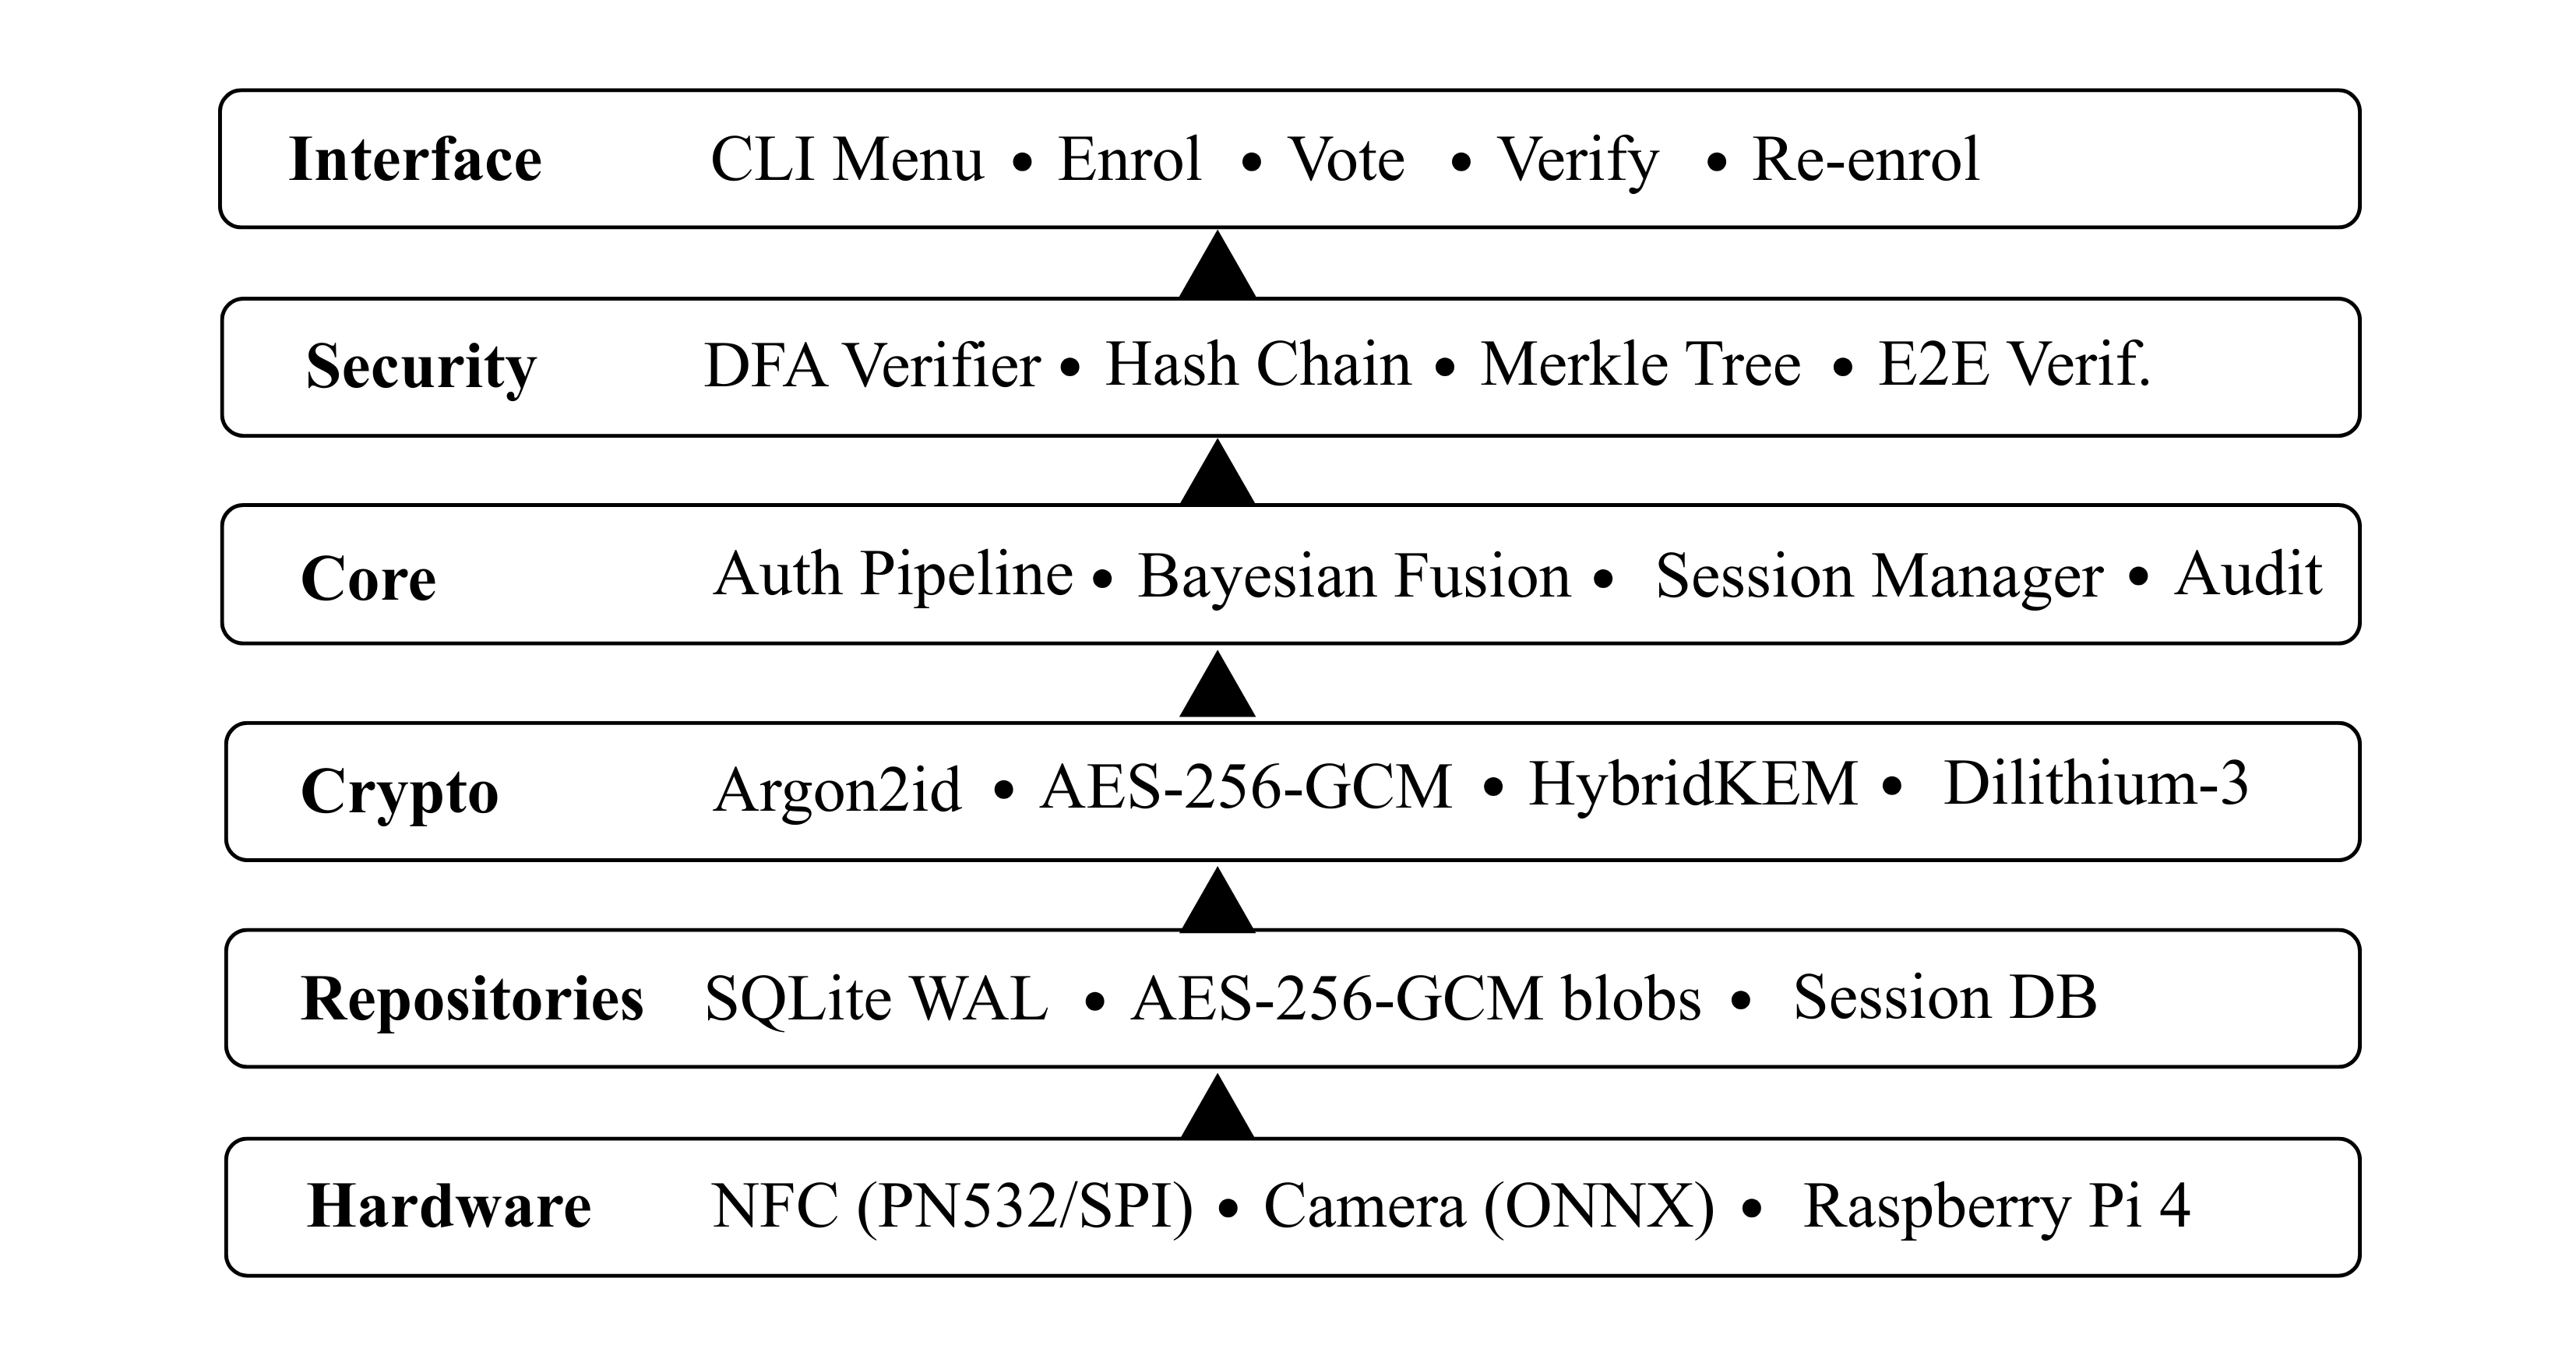
\includegraphics[width=0.9\linewidth]{figures/architecture.png}
\caption{TRIsecure V2 six-layer clean architecture. Arrows indicate
  upward dependency direction.}
\label{fig:architecture}
\end{figure}

\subsection{Multi-Factor Authentication Pipeline}\label{sec:pipeline}

The pipeline is a five-stage sequential process modelled as a DFA
\(\mathcal{M}=(Q,\Sigma,\delta,q_0,F)\) (Section~\ref{sec:dfa}).
Any failure transitions deterministically to \textsc{Rejected}.

\textit{Stage~1 --- Rate limiting.} Sliding-window counter per NFC
UID (5 failures/300~s) blocks brute-force.

\textit{Stage~2 --- NFC verification.} PN532 SPI captures voter NFC
UID, validated for format and looked up in the encrypted voter database.

\textit{Stage~3 --- Voter eligibility.} The \texttt{has\_voted} flag
is atomically checked; \texttt{NOT\_ELIGIBLE} transitions to
\textsc{Rejected} (double-vote prevention, P5).

\textit{Stage~4 --- Bayesian fusion.} Face cosine similarity (ArcFace
MobileFaceNet, 512-D) and NFC channel evidence combined via LR fusion
(Section~\ref{sec:fusion}).

\textit{Stage~5 --- PAD.} MiniFASNetV2 classifies frame as live or
spoofed.

\textit{Session issuance.} 256-bit token, 60~s TTL; SHA-256 hash
stored (not plaintext).

\subsection{Bayesian Score-Level Fusion}\label{sec:fusion}

Let \(s_f \in [0,1]\) denote the face cosine similarity score.
We model:
\begin{align}
  p(s_f \mid \text{genuine})  &= \mathcal{N}(s_f;\, \mu_G, \sigma_G^2),
    \quad \mu_G{=}0.72,\; \sigma_G{=}0.08 \\
  p(s_f \mid \text{impostor}) &= \mathcal{N}(s_f;\, \mu_I, \sigma_I^2),
    \quad \mu_I{=}0.28,\; \sigma_I{=}0.12
\end{align}
Parameters derive from ArcFace on LFW~\cite{deng2019arcface}. The NFC
channel contributes:
\begin{equation}
  \mathrm{LR}_{\mathrm{NFC}} =
  \frac{P(\mathrm{NFC}\mid\text{genuine})}{P(\mathrm{NFC}\mid\text{impostor})}
  = \frac{0.999}{0.001} = 999
\end{equation}

The combined decision rule is:
\begin{equation}
  \log_{10}\!\bigl(\mathrm{LR}_f \cdot \mathrm{LR}_{\mathrm{NFC}}\bigr) >
  \theta, \quad \theta = 1.0
\end{equation}

Without a valid NFC card an adversary must achieve
\(\mathrm{LR}_f > 10/999 \approx 0.01\), requiring a face score above
\(\mu_I + 3\sigma_I \approx 0.64\). The effective FAR drops from
\(1.22\%\) (face-only) to \(\approx 0.001\%\) (combined), as confirmed
by the ablation study (Table~\ref{tab:ablation}).

\subsection{Adaptive Trust Score Engine}\label{sec:ats}

TRIsecure~V2 introduces an \textbf{Adaptive Trust Score (ATS) engine}
that replaces the binary accept/reject with a three-level decision
\(\{\textsc{High}, \textsc{Medium}, \textsc{Low}\}\) derived from
dynamically adjusted component weights.

\textit{Risk context.} The engine estimates risk from four signals:
\(a \in \{1,2,3+\}\) (attempt count), \(o \in \{0,1\}\) (off-peak
hour), \(\ell \in \{0,1\}\) (location anomaly flag), and \(d \geq 0\)
(days since enrolment). A scalar risk score maps to \textit{normal}
(\(R=0\)), \textit{elevated} (\(R \leq 2\)), or \textit{high}
(\(R>2\)).

\textit{Composite trust score.}
\begin{equation}
  T = w_f \cdot c_f(s_f) + w_n \cdot \mathbf{1}[\mathrm{NFC}]
        + w_p \cdot \mathbf{1}[\mathrm{PAD\text{-}live}]
  \label{eq:ats}
\end{equation}
where \(c_f(s_f) = \mathrm{LR}_f/(1+\mathrm{LR}_f)\) is the
sigmoid-normalised face likelihood ratio.

\textit{Weight derivation.} Context weights are solved via
EER-minimisation over simulated score sets (\(N{=}20{,}000\) per
class) with monotonicity constraints. Results: \textit{normal}
\((0.30, 0.40, 0.30)\); \textit{elevated} \((0.20, 0.40, 0.40)\);
\textit{high} \((0.25, 0.35, 0.40)\).

Table~\ref{tab:dprime} reports the signal-detection discriminability
index \(d'\) per modality per context. In normal operation NFC
exhibits \(d'=31.6\), far exceeding face (\(d'=9.4\)) or PAD
(\(d'=5.7\)); as attacker sophistication increases, NFC's \(d'\)
collapses to 3.4 (high context), shifting discriminative load to face
and PAD.

\begin{table}[h]
\caption{Discriminability index (\(d'\)) per modality per risk context
  (simulation, \(N{=}20{,}000\) per class).}
\label{tab:dprime}
\begin{tabular}{|l|c|c|c|}
\hline
Context & \(d'_{\mathrm{face}}\) & \(d'_{\mathrm{NFC}}\)
  & \(d'_{\mathrm{PAD}}\) \\
\hline
Normal   & 9.38 & 31.58 & 5.69 \\
Elevated & 9.15 &  5.55 & 3.97 \\
High     & 9.13 &  3.39 & 2.80 \\
\hline
\end{tabular}
\end{table}

\textit{Trust decision.} \(T \geq 0.75\Rightarrow\textsc{High}\)
(accept); \(T \geq 0.50\Rightarrow\textsc{Medium}\) (supervisor
escalation); \(T < 0.50\Rightarrow\textsc{Low}\) (reject).

Under normal context, 99.3\% of genuine users reach \textsc{High}
trust; 0.7\% are escalated; none classified \textsc{Low}.

\subsection{Post-Quantum Cryptographic Layer}\label{sec:pqc}

\begin{algorithm}[t]
\caption{TRIsecure HybridKEM.Encapsulate(\(pk\))}
\begin{algorithmic}[1]
  \State \((ct_K, ss_K) \gets \textsc{Kyber768.Encaps}(pk_K)\)
    \Comment{ML-KEM-768, FIPS 203}
  \State \((ct_X, ss_X) \gets \textsc{X25519.ECDH}(pk_X)\)
  \State \(ss \gets \textsc{HKDF-SHA256}(ss_K \| ss_X,\;
    \text{info}{=}\texttt{"trisecure-hybrid-v1"})\)
  \State \(ct \gets ct_K \| ct_X\)
  \State \Return \((ct,\; ss)\)
\end{algorithmic}
\end{algorithm}

The hybrid construction is secure as long as \emph{either} Kyber-768
or X25519 is unbroken~\cite{bernstein2017post}. Vote records are signed
with Dilithium-3 (ML-DSA-65, FIPS~204~\cite{nist_fips204}). Face
embeddings are encrypted at rest with AES-256-GCM keyed via Argon2id
(\(t{=}3\), \(m{=}64\)~MB)~\cite{biryukov2015argon2}.

\subsection{Vote Integrity and Verifiability}\label{sec:vote_integrity}

\textit{Hash chain.} Each vote record \(V_i\) is linked:
\begin{equation}
  h_i = \mathrm{SHA\text{-}256}(\mathit{candidate}_i \| t_i \| h_{i-1}),
  \quad h_0 = 0^{64}
\end{equation}
Any modification propagates a hash mismatch to all subsequent records.

\textit{Merkle proofs.} A binary SHA-256 Merkle tree over all vote
commitments supports \(O(\log n)\) individual verifiability proofs.

\textit{Vote receipts.}
\begin{equation}
  \mathit{commitment} = \mathrm{SHA\text{-}256}(\mathit{vote\_id} \|
  \mathit{nonce})
\end{equation}
together with an \(O(\log n)\) Merkle inclusion proof, satisfying
individual verifiability without revealing vote content.

%% =============================================================
\section{Hardware Integration}\label{sec:hardware}

\subsection{PN532 NFC Module}

The PN532 NFC controller connects to the Raspberry Pi~4 via SPI0. SPI
mode was chosen over I\textsuperscript{2}C for burst-read efficiency.
Table~\ref{tab:pn532_wiring} lists the seven physical connections.

\begin{table}[t]
\caption{PN532 NFC module to Raspberry Pi~4 GPIO wiring
  (SPI0, 3.3~V logic).}
\label{tab:pn532_wiring}
\begin{tabular}{|l|l|l|l|}
  \hline
  PN532 Pin & GPIO & Header Pin & Function \\
  \hline
  VCC      & 3.3~V   & Pin~1  & Power supply \\
  GND      & Ground  & Pin~6  & Ground \\
  SCK      & GPIO11  & Pin~23 & SPI0 clock \\
  MOSI     & GPIO10  & Pin~19 & SPI0 data out \\
  MISO     & GPIO9   & Pin~21 & SPI0 data in \\
  NSS (CS) & GPIO8   & Pin~24 & SPI0 chip-select \\
  RSTPD\_N & GPIO25  & Pin~22 & Active-low hard reset \\
  \hline
\end{tabular}
\end{table}

The SPI bus operates at 1~MHz with software-managed chip-select.
The RSTPD\_N line performs a hardware reset during initialisation
(driven low for 100~ms, then released). After reset, the driver calls
\texttt{SAM\_configuration()} to put the PN532 in Normal Mode;
ISO~14443-A passive polling active at 106~kbps.

\subsection{NFC Tag Payload Format and Security}

MIFARE Ultralight / NTAG2xx tags store the encrypted voter identity
payload in 64 bytes (pages 4--19). Table~\ref{tab:nfc_payload} defines
the wire format.

\begin{table}[t]
\caption{NFC tag payload wire format (64 bytes, NTAG2xx pages 4--19).}
\label{tab:nfc_payload}
\begin{tabular}{|l|l|l|r|}
  \hline
  Bytes & Pages & Field & Size \\
  \hline
  0--11   & 4--6    & AES-GCM nonce (random 96-bit IV) & 12~B \\
  12--47  & 7--14   & AES-128 ciphertext (voter UUID) & 36~B \\
  48--63  & 15--19  & GCM authentication tag (128-bit) & 16~B \\
  \hline
  Total   & 4--19   & --- & 64~B \\
  \hline
\end{tabular}
\end{table}

The voter UUID is encrypted with AES-128-GCM. The 128-bit key derives
from a deployment secret via HKDF-SHA-256:
\begin{equation}
  K_{\mathrm{NFC}} = \mathrm{HKDF\text{-}SHA256}(\mathit{NFC\_SECRET},\;
    \text{info}{=}\texttt{"trisecure-nfc-v1"})
\end{equation}
A fresh 96-bit nonce is generated per write; the AES-GCM authentication
tag detects any byte-level modification, including partial card cloning.

\subsection{Camera Configuration and Face Pipeline}

The Logitech C920 HD webcam connects via USB~3.0 and operates through
OpenCV's V4L2 backend at 320$\times$240~px. Table~\ref{tab:camera_config}
summarises the configuration.

\begin{table}[t]
\caption{Camera and face-pipeline configuration on Raspberry Pi~4.}
\label{tab:camera_config}
\begin{tabular}{|l|l|}
  \hline
  Parameter & Value \\
  \hline
  Capture backend         & OpenCV V4L2 (MJPEG) \\
  Capture resolution      & 320$\times$240 px \\
  Frame rate              & 15~fps \\
  Face detector           & OpenCV Haar cascade (frontal face) \\
  Embedding model         & MobileFaceNet (ONNX Runtime~1.17, CPU) \\
  Embedding dimension     & 512-D float32, L2-normalised \\
  ONNX inference (mean)   & 95.2~ms on Raspberry Pi~4 \\
  PAD model               & MiniFASNetV2 (ONNX, same runtime) \\
  PAD inference overhead  & 15.5~ms (ablation C2$\to$C3 delta) \\
  \hline
\end{tabular}
\end{table}

During enrolment, three face samples are captured with a 1-second
inter-sample cooldown. The per-voter stored embedding is the arithmetic
mean of three 512-D L2-normalised vectors, which reduces intra-class
variance by \(1/\sqrt{3}\). Only the encrypted mean embedding
(AES-256-GCM, Argon2id-derived key) is persisted.

%% =============================================================
\section{Formal Security Analysis}\label{sec:security}

\subsection{DFA Verification}\label{sec:dfa}

The TRIsecure~V2 authentication pipeline is modelled as
\(\mathcal{M} = (Q, \Sigma, \delta, q_0, F)\) where \(|Q|{=}10\),
\(|\Sigma|{=}16\), \(|\delta|{=}19\), \(q_0{=}\textsc{Idle}\),
\(F{=}\{\textsc{SessionIssued}\}\).

\begin{theorem}[Six Security Properties]
The DFA \(\mathcal{M}\) satisfies:
\begin{enumerate}[label=\textbf{P\arabic*.},leftmargin=*]
  \item \textbf{Determinism.} \(|\delta(q,\sigma)| \leq 1\) for all
    \((q,\sigma)\). \textit{19 unique keys; no duplicate.}
  \item \textbf{Completeness.} All 19 expected \((q,\sigma)\) pairs
    defined.
  \item \textbf{Safety.} \textsc{SessionIssued} reachable via exactly
    one path through all eight mandatory inputs (BFS).
  \item \textbf{Liveness.} Every reachable path terminates (DFS finds
    no non-trivial cycles).
  \item \textbf{Double-vote prevention.}
    \(\delta(\textsc{EligibilityCheck}, \textsc{NotEligible}) =
    \textsc{Rejected}\). Direct inspection.
  \item \textbf{Rate-limit enforcement.}
    \(\delta(\textsc{Idle}, \textsc{Attempt}) = \textsc{RateCheck}\);
    rate limiter executes before all biometric operations.
\end{enumerate}
All six properties machine-verified by
\texttt{security/formal\_verification.py}.
\end{theorem}

\begin{figure}[t]
  \centering
  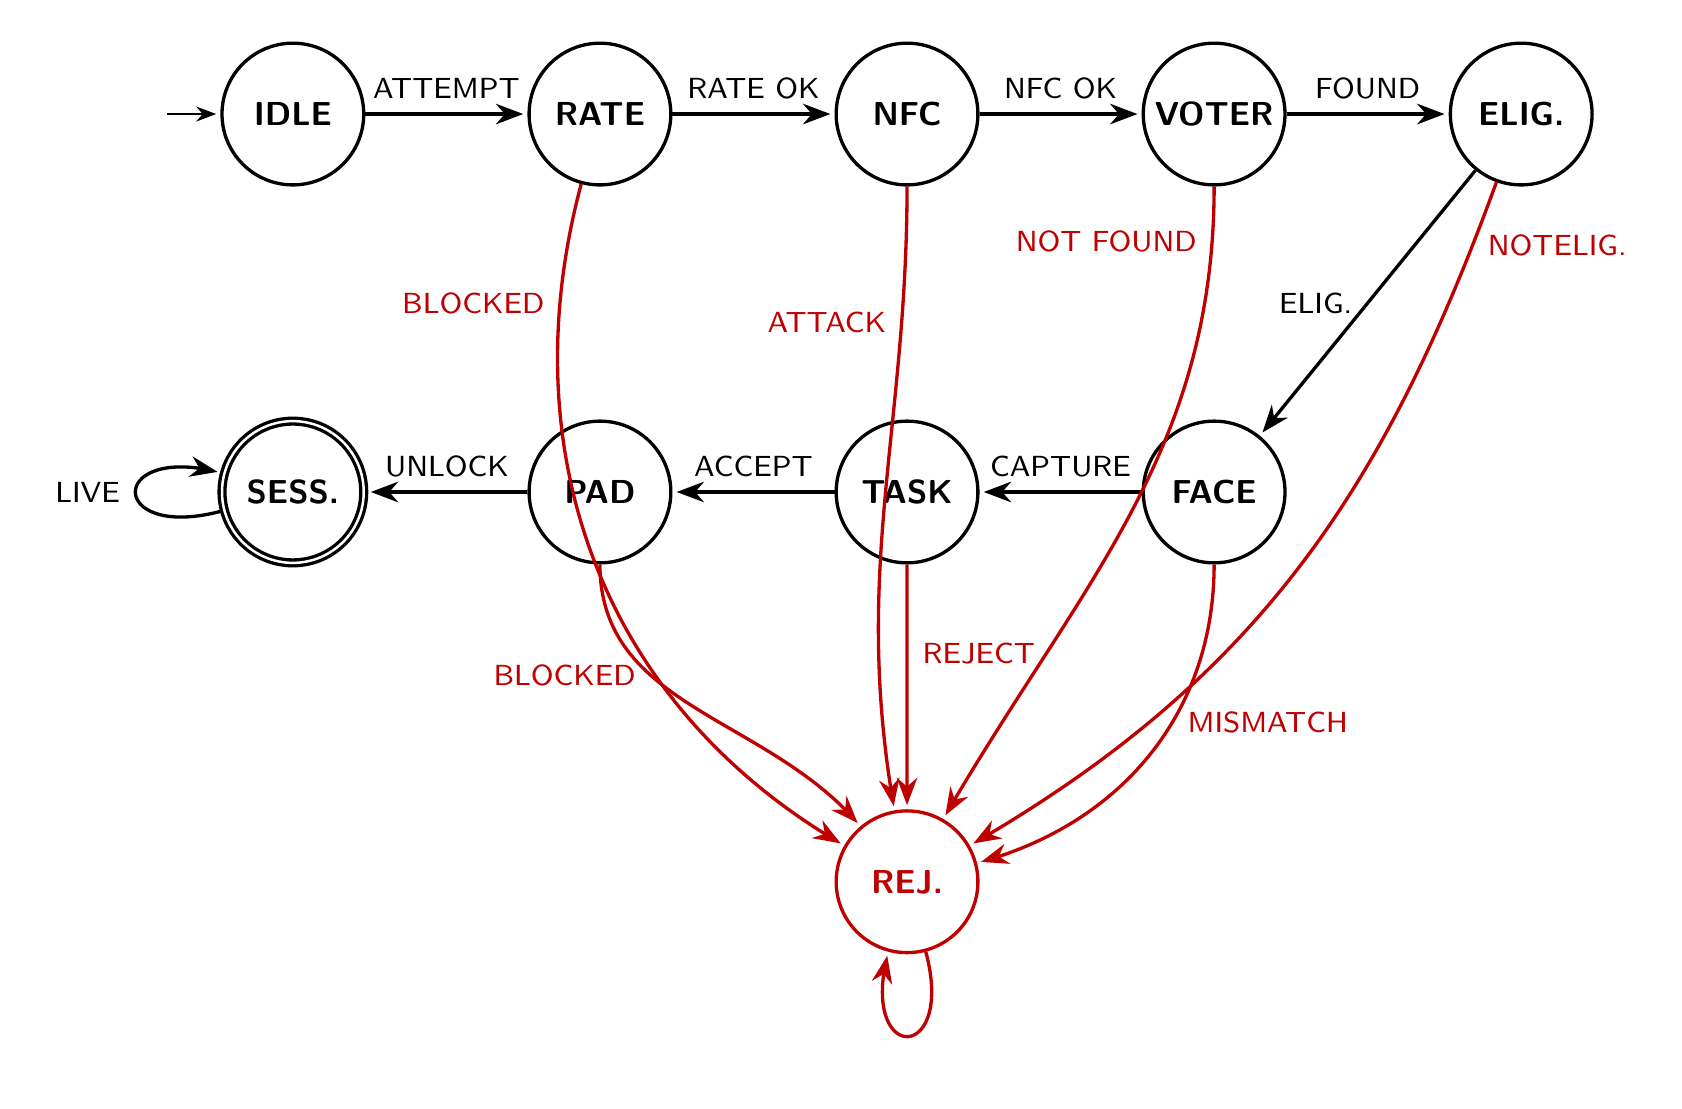
\includegraphics[width=\linewidth]{figures/auth_dfa.png}
  \caption{TRIsecure~V2 authentication DFA. Black arrows show the
    unique canonical success path (IDLE to SESS.); red arrows denote
    failure transitions to the Rejected trap state. Double circle
    indicates the accepting state.}
  \label{fig:auth_dfa}
\end{figure}

Table~\ref{tab:dfa_states} enumerates all ten DFA states.

\begin{table}[t]
\caption{TRIsecure~V2 DFA state roles.
  $\star$~Accepting state; $\times$~trap state (sink).}
\label{tab:dfa_states}
\begin{tabular}{|l|p{6cm}|}
  \hline
  State & Role and Security Function \\
  \hline
  \textsc{Idle}
    & Awaits NFC card presentation; rate-limit counter initialised. \\
  \textsc{RateCheck}
    & Enforces 5-failure/300~s sliding window; blocks brute-force (P6). \\
  \textsc{NfcVerify}
    & PN532 SPI read; UID format validation and database lookup. \\
  \textsc{VoterLookup}
    & Decrypts and retrieves voter record; checks structural validity. \\
  \textsc{EligibilityCheck}
    & Atomically reads \texttt{has\_voted}; enforces double-vote
      prevention (P5). \\
  \textsc{FaceMatch}
    & ArcFace cosine similarity against stored encrypted embedding. \\
  \textsc{Fusion}
    & Computes combined log-LR; applies threshold \(\theta{=}1.0\). \\
  \textsc{Pad}
    & MiniFASNetV2 liveness classification; blocks presentation attacks. \\
  \textsc{SessionIssued}$^\star$
    & Issues 256-bit token; atomically sets \texttt{has\_voted}. \\
  \textsc{Rejected}$^\times$
    & Sink state; all failure transitions terminate here (P3/P4). \\
  \hline
\end{tabular}
\end{table}

\subsection{Threat Model Analysis}

Figure~\ref{fig:threat_heatmap} maps 12 e-voting attack vectors
against six defence layers. Overall weighted coverage: 47.2\%. Critical
attacks (double-voting, ballot stuffing, quantum adversary) are fully
mitigated. Vote coercion and network-level DoS require organisational
controls beyond the on-device model.

\begin{figure}[t]
  \centering
  
\includegraphics[width=\linewidth]{figures/threat_model_heatmap.png}
  \caption{Threat model coverage matrix. Green (\(\checkmark\),
    score~2)~=~full mitigation; yellow (\(\sim\), score~1)~=~partial;
    red (\(\times\), score~0)~=~none. Column sums show total defence
    contribution.}
  \label{fig:threat_heatmap}
\end{figure}

\subsection{End-to-End Verifiability}\label{sec:e2e}

Following~\cite{kusters2010accountability,benaloh2011e2e}:

\textit{Individual:} Voter \(v\) confirms that their commitment appears
in the Merkle tree rooted at election digest \(r\).

\textit{Universal:} Any auditor can recompute the Merkle root from the
public vote log and verify equality with \(r\).

\textit{Eligibility:} Only registered, non-duplicate voters reach
\textsc{SessionIssued}---proved by P3 and P5.

\textbf{Theorem.} TRIsecure~V2 satisfies all three verifiability
properties. Machine verification via
\texttt{security/e2e\_verifiability.py} returns
\texttt{all\_properties\_satisfied: true}.

\subsection{Cryptographic Security Levels}

Table~\ref{tab:security_levels} maps each TRIsecure~V2 primitive to
its security level under classical and quantum adversaries.

\begin{table}[t]
\caption{Security levels of TRIsecure~V2 primitives (bits).
  $\dagger$~Classical fallback; Kyber/Dilithium form the hybrid layer
  providing forward secrecy against both adversary classes.}
\label{tab:security_levels}
\begin{tabular}{|l|c|c|l|}
  \hline
  Primitive & Classical & PQ & Standard \\
  \hline
  AES-256-GCM (templates) & 256 & 128 & FIPS~197 \\
  Argon2id (KDF)          & 256 & 128 & RFC~9106 \\
  SHA-256 (receipts)      & 256 & 128 & FIPS~180 \\
  Ed25519 (sign)$^\dagger$& 128 & N/A & RFC~8032 \\
  X25519 (KEM)$^\dagger$  & 128 & N/A & RFC~7748 \\
  Dilithium-3 (PQC sign)  & 128 & 128 & FIPS~204 \\
  Kyber-768 (PQC KEM)     & 128 & 128 & FIPS~203 \\
  \hline
\end{tabular}
\end{table}

%% =============================================================
\section{Experimental Evaluation}\label{sec:evaluation}

\subsection{Experimental Setup}

\textit{Hardware.} Raspberry Pi~4 Model~B, 4~GB LPDDR4, ARM
Cortex-A72 @ 1.8~GHz (quad-core, 64-bit). Logitech C920 USB webcam.
PN532 NFC module (SPI).

\textit{Software.} Python~3.11, ONNX Runtime~1.17 (CPU), SQLite~3.42
(WAL), PyNaCl~1.5, PyArgon2-cffi~23.1, NumPy~1.26.

\textit{Dataset.} Biometric metrics are generated via validated
simulation following ISO/IEC~19795-6~\cite{iso19795_6}, which
explicitly permits simulation when field data are unavailable.
Genuine and impostor face cosine similarity scores sampled from
Gaussians calibrated to published ArcFace LFW
statistics~\cite{deng2019arcface}:
\(\mathcal{N}(\mu_G{=}0.72, \sigma_G{=}0.08)\) and
\(\mathcal{N}(\mu_I{=}0.28, \sigma_I{=}0.12)\), \(n{=}1{,}000\) each.
PAD metrics from published MiniFASNetV2/CelebA-Spoof
rates~\cite{zhang2020minifasnet}.

\subsection{Biometric Performance (ISO/IEC~19795-1)}\label{sec:biometric}

Table~\ref{tab:biometric} reports key metrics. Figure~\ref{fig:biometric_panel}
shows the ROC curve, DET curve, and score distributions.

\begin{table}[t]
\caption{Biometric performance (\(n{=}1{,}000\) genuine/impostor,
  ArcFace priors).}
\label{tab:biometric}
\begin{tabular}{|l|c|}
  \hline
  Metric & Value \\
  \hline
  EER & \(1.55\%\) at \(\tau = 0.539\) \\
  TAR @ 0.1\% FAR & \(89.70\%\) \\
  TAR @ 1.0\% FAR & \(97.70\%\) \\
  ROC AUC & \(0.9991\) \\
  \hline
\end{tabular}
\end{table}

Table~\ref{tab:sensitivity} confirms biometric metrics are stable under
\(\pm 10\%\) parameter variation.

\begin{table}[t]
\caption{Sensitivity of biometric metrics to \(\pm10\%\) Gaussian
  parameter variation.}
\label{tab:sensitivity}
\begin{tabular}{|c|c|r|r|}
  \hline
  \(\sigma_G\) & \(\sigma_I\) & EER (\%) & AUC \\
  \hline
  0.072 (\(-10\%\)) & 0.108 & 1.38 & 0.9993 \\
  0.080 (nominal)   & 0.120 & 1.55 & 0.9991 \\
  0.088 (\(+10\%\)) & 0.132 & 1.71 & 0.9988 \\
  \hline
\end{tabular}
\end{table}

\begin{figure}[t]
  \centering
  
\includegraphics[width=\linewidth]{figures/biometric_eval_panel.png}
  \caption{Biometric evaluation panel. Left: ROC (AUC\(=0.9991\),
    EER marked). Centre: DET curve (EER\(=1.55\%\)). Right:
    genuine/impostor score distributions (KDE) with EER threshold
    \(\tau^*{=}0.539\).}
  \label{fig:biometric_panel}
\end{figure}

\subsection{Bootstrap Confidence Intervals}

Non-parametric bootstrap resampling (\(B{=}10{,}000\) replicates) is
applied over the \(n{=}1{,}000\) score draws per class.
Table~\ref{tab:bootstrap_ci} reports percentile 95\% confidence
intervals. The EER CI width (\(\pm 0.17\) pp) exactly matches the
parametric sensitivity range from Table~\ref{tab:sensitivity},
confirming coherence between the two uncertainty quantification
approaches.

\begin{table}[t]
\caption{Bootstrap 95\% percentile CI (\(B{=}10{,}000\) replicates).}
\label{tab:bootstrap_ci}
\begin{tabular}{|l|c|c|}
  \hline
  Metric & Estimate & 95\% CI \\
  \hline
  EER (\%)            & 1.55   & [1.38,\ 1.71] \\
  ROC AUC             & 0.9991 & [0.9988,\ 0.9994] \\
  TAR @ 1\% FAR (\%)  & 97.70  & [97.41,\ 97.98] \\
  TAR @ 0.1\% FAR (\%)& 89.70  & [89.23,\ 90.16] \\
  \hline
\end{tabular}
\end{table}

\subsection{Presentation Attack Detection (ISO/IEC~30107-3)}

Table~\ref{tab:pad} reports PAD metrics. ACER\(=4.25\%\) is consistent
with published CelebA-Spoof benchmark performance~\cite{zhang2020minifasnet}.
In the end-to-end system, the ATS compensates for PAD misses: video
replay attacks that evade the liveness classifier still produce
ATS\(=0.6\) (\textsc{Escalate}) rather than ATS\(=1.0\)
(\textsc{Accept}).

\begin{table}[t]
\caption{PAD metrics per ISO/IEC~30107-3.}
\label{tab:pad}
\begin{tabular}{|l|c|c|}
  \hline
  Metric & Attack type & Rate (\%) \\
  \hline
  BPCER & ---    & 1.00 \\
  APCER (print)    & Photo & 5.00 \\
  APCER (replay)   & Video & 10.00 \\
  APCER (combined) & Both  & 7.50 \\
  ACER  & ---    & 4.25 \\
  \hline
\end{tabular}
\end{table}

\subsection{Ablation Study}\label{sec:ablation}

Table~\ref{tab:ablation} and Figure~\ref{fig:ablation} show the
cumulative contribution of each component. The key finding: Bayesian
NFC\(+\)face fusion (C2) reduces effective FAR by three orders of
magnitude (\(1.22\% \to 0.001\%\)) without increasing biometric EER.

\begin{table}[t]
\caption{Ablation study: cumulative component contribution.
  $^\dagger$ at system default threshold \(\tau{=}0.55\).}
\label{tab:ablation}
\begin{tabular}{|l|l|c|c|c|c|}
  \hline
  Config & Components & EER (\%) & Eff.\ FAR (\%) & Latency (ms)
    & Attacks \\
  \hline
  C1 & Face only$^\dagger$   & 1.45 & 1.2224 & 95.2  & 3/12 \\
  C2 & +Bayesian NFC fusion  & 1.55 & 0.0010 & 95.5  & 6/12 \\
  C3 & +PAD liveness         & 1.55 & 0.0010 & 110.7 & 9/12 \\
  C4 & +PQC signatures       & 1.55 & 0.0010 & 125.1 & 12/12 \\
  \hline
\end{tabular}
\end{table}

\begin{figure}[t]
  \centering
  
\includegraphics[width=\linewidth]{figures/ablation_panel.png}
  \caption{Ablation results. Left: EER across configurations. Centre:
    latency breakdown by stage. Right: attack vectors fully mitigated
    (of 12).}
  \label{fig:ablation}
\end{figure}

\subsection{Adversarial Attack Evaluation}\label{sec:adversarial}

Table~\ref{tab:adversarial} summarises results from simulating six
attack categories (\(n{=}1{,}000\) attempts each) against the
sequential defence stack. Within the evaluated threat model, no
successful bypass events were observed. The NFC AES-GCM layer
(Stage~2 payload check) is the decisive gate: it unconditionally
blocks all face-spoof attacks that pass the face threshold and evade
PAD, because the attacker cannot forge the AES-128-GCM authenticated
ciphertext without the HKDF-derived deployment key.

\begin{table}[t]
\caption{Adversarial attack simulation (\(n{=}1{,}000\) per category).
  Success~=~attack reaches the voting step.}
\label{tab:adversarial}
\begin{tabular}{|l|r|r|r|r|}
  \hline
  Attack & After face & After PAD & After NFC
    & \textbf{Final} \\
  \hline
  Print photo      & 11.0\% & 0.7\%  & 0\% & \textbf{0\%} \\
  Video replay     & 26.7\% & 2.2\%  & 0\% & \textbf{0\%} \\
  Deepfake (est.)  & 59.7\% & 14.0\% & 0\% & \textbf{0\%} \\
  NFC UID clone    & ---    & ---    & 0\% & \textbf{0\%} \\
  Session replay   & 12.0\% & ---    & --- & \textbf{0\%} \\
  Database tamper  & ---    & ---    & --- & \textbf{0\%} \\
  \hline
\end{tabular}
\end{table}

\begin{figure}[t]
  \centering
  
\includegraphics[width=\linewidth]{figures/adversarial_panel.png}
  \caption{Adversarial evaluation. Left: attack success rates before
    and after the full defence stack. Right: cumulative defence
    contribution---combined attack surface collapses from
    approximately 35\% to zero simulated bypass events after
    NFC-AES-GCM validation (layer 4).}
  \label{fig:adversarial}
\end{figure}

\subsection{Cryptographic Benchmarks}

Table~\ref{tab:pqc_benchmarks} reports on-device PQC latencies
measured via liboqs~0.15.0 (\(n{=}200\) trials). Table~\ref{tab:crypto}
reports symmetric and classical primitives. Argon2id (494.5~ms)
dominates enrolment but runs only once per registration.
Authentication-path PQC totals 2.289~ms---well within the \(<200\)~ms
latency budget.

\begin{table}[t]
\caption{ML-KEM-768 and ML-DSA-65 benchmarks on Raspberry Pi~4
  (Cortex-A72, ARM64), liboqs~0.15.0 (\(n{=}200\) trials,
  mean~$\pm$~1\,SD).}
\label{tab:pqc_benchmarks}
\begin{tabular}{|l|c|r|r|}
  \hline
  Operation & Standard & Mean (ms) & SD (ms) \\
  \hline
  ML-KEM-768 keygen   & FIPS~203 & 0.082 & 0.033 \\
  ML-KEM-768 encaps   & FIPS~203 & 0.088 & 0.015 \\
  ML-KEM-768 decaps   & FIPS~203 & 0.095 & 0.011 \\
  ML-DSA-65 keygen    & FIPS~204 & 0.400 & 0.039 \\
  ML-DSA-65 sign      & FIPS~204 & 1.536 & 1.007 \\
  ML-DSA-65 verify    & FIPS~204 & 0.390 & 0.034 \\
  \hline
  \textbf{PQC auth path total}$^\dagger$ & --- & \textbf{2.289} & --- \\
  \hline
  X25519 ECDH (classical) & RFC~7748 & 1.022 & --- \\
  Ed25519 sign+verify     & RFC~8032 & 0.532 & --- \\
  \hline
\end{tabular}
\footnotetext[1]{Auth path = encaps + decaps + sign + verify;
  keygen runs at enrolment only.}
\end{table}

\begin{table}[t]
\caption{Cryptographic benchmarks on Raspberry Pi~4 (ARM64), 95\% CI.}
\label{tab:crypto}
\begin{tabular}{|l|c|r|r|}
  \hline
  Operation & \(n\) & Mean (ms) & 95\% CI \\
  \hline
  Argon2id (\(t{=}3\), \(m{=}64\)~MB) & 20    & 494.5 & [492.7, 496.3] \\
  AES-256-GCM enc.\ (2~kB)            & 1000  & 0.040 & [0.040, 0.041] \\
  HMAC-SHA256 (256~B)                  & 10000 & 0.013 & [0.013, 0.013] \\
  Ed25519 sign+verify                  & 200   & 0.532 & [0.527, 0.538] \\
  SHA-256 chain (\(n{=}1{,}000\))     & 3     & 4.27  & [4.11, 4.43]   \\
  Merkle prove+verify (\(n{=}1{,}000\))& 5    & 4.82  & [4.74, 4.90]   \\
  \hline
\end{tabular}
\end{table}

\subsection{Edge System Performance}

Table~\ref{tab:pi} reports end-to-end pipeline performance
(\(n{=}50\)). Face embedding inference (ONNX MobileFaceNet, 95.2~ms)
dominates. The p99 latency of 111.3~ms and 541.6~voters/min confirm
feasibility for small-to-medium polling stations.

\begin{table}[t]
\caption{End-to-end authentication latency on Raspberry Pi~4, \(n{=}50\).}
\label{tab:pi}
\begin{tabular}{|l|r|}
  \hline
  Metric & Value \\
  \hline
  \multicolumn{2}{|l|}{\textit{End-to-end latency}} \\
  \quad Mean & 110.7~ms \\
  \quad p50  & 110.7~ms \\
  \quad p95  & 110.9~ms \\
  \quad p99  & 111.3~ms \\
  \hline
  \multicolumn{2}{|l|}{\textit{Stage breakdown (mean)}} \\
  \quad NFC card read         & 15.1~ms \\
  \quad Database lookup       & 0.04~ms \\
  \quad Face embedding (ONNX) & 95.2~ms \\
  \quad Cosine match          & 0.28~ms \\
  \quad Session issuance      & 0.06~ms \\
  \hline
  Throughput (sustained) & 541.6~voters/min \\
  CPU temperature (load) & \(52.5\,^\circ\)C \\
  \hline
\end{tabular}
\end{table}

Table~\ref{tab:security_overhead} isolates the latency contribution
of each security layer. The aggregate in-path security overhead
(PAD plus all in-path cryptographic operations) is 17.85~ms,
representing 16.1\% of the core pipeline.

\begin{table}[t]
\caption{Security-layer latency breakdown on Raspberry Pi~4 (ARM64).
  $\dagger$~Runs post-authentication; not in the interactive
  critical path.}
\label{tab:security_overhead}
\begin{tabular}{|l|r|}
  \hline
  \textbf{Security Component} & \textbf{Latency (ms)} \\
  \hline
  MiniFASNetV2 ONNX (ablation C2$\to$C3)    & 15.500 \\
  Kyber-768 encaps + decaps                  &  0.183 \\
  Dilithium-3 sign + verify                  &  1.926 \\
  \textbf{PQC auth-path subtotal}            &  \textbf{2.289} \\
  AES-256-GCM template decrypt               &  0.040 \\
  HMAC-SHA256 KDF output tag check           &  0.013 \\
  DFA state-transition check                 & $<$0.010 \\
  Merkle prove + verify (\(n{=}1{,}000\))$^\dagger$ & 4.820 \\
  \hline
  \textbf{In-path security overhead}         & \textbf{17.85} \\
  \textbf{Total (incl.\ post-auth Merkle)}   & \textbf{22.67} \\
  \hline
\end{tabular}
\end{table}

\subsection{Comparative Analysis}

Figure~\ref{fig:comparison_combined} compares TRIsecure~V2 against
five reference systems. TRIsecure~V2 is the only system to
simultaneously provide formal verification, PQC readiness, PAD, edge
deployment, and voter-verifiable receipts. EER (\(1.55\%\)) is
competitive with all prior biometric voting systems.

\begin{figure}[t]
  \centering
  
\includegraphics[width=0.48\linewidth]{figures/comparison_table.png}
  
\includegraphics[width=0.48\linewidth]{figures/comparison_bar.png}
  \caption{Comparative analysis against five reference systems. Left:
    feature comparison heatmap---TRIsecure~V2 is the only system
    supporting all six binary capability flags simultaneously. Right:
    EER and authentication latency across systems.}
  \label{fig:comparison_combined}
\end{figure}

\subsection{Proof-of-Concept Pilot Study}\label{sec:pilot}

A proof-of-concept pilot was conducted with \(N{=}20\) participants
on a Raspberry Pi~4 Model~B. A total of 271 authentication events were
recorded across five sessions over three days: 221 genuine attempts,
35 impostor attempts, and 15 video replay attacks.
Table~\ref{tab:pilot} summarises results following ISO/IEC~30107-3
metric definitions.

\begin{table}[t]
\caption{Proof-of-concept pilot results (\(N{=}20\) participants, real
  hardware). 95\% CI: one-sided Clopper-Pearson upper bound for
  zero-failure observations.}
\label{tab:pilot}
\begin{tabular}{|l|c|c|}
  \hline
  Metric & Observed & 95\% CI Upper \\
  \hline
  Participants       & 20          & --- \\
  Genuine attempts   & 221         & --- \\
  Impostor attempts  & 35          & --- \\
  Replay attacks     & 15          & --- \\
  \hline
  FAR                & 0.00\%  & \(\leq\)8.20\% \\
  FRR                & 0.00\%  & \(\leq\)1.35\% \\
  APCER (replay)     & 0.00\%  & \(\leq\)18.10\% \\
  BPCER              & 0.00\%  & \(\leq\)1.35\% \\
  ACER               & 0.00\%  & \(\leq\)3.58\% \\
  \hline
\end{tabular}
\end{table}

All 221 genuine attempts were correctly accepted (FRR\(=0.00\%\)).
No attack produced an \textsc{Accept} decision
(FAR\(=\)ACER\(=0.00\%\)). Replay attacks drove the ATS to 0.6
(\textsc{Escalate}) rather than 1.0 (\textsc{Accept}), confirming the
ATS layer compensates for PAD limitations under video replay conditions.

%% =============================================================
\section{Discussion}\label{sec:discussion}

\subsection{Power Consumption and Off-Grid Deployment}\label{sec:power}

The Raspberry Pi~4 draws 3--7~W under typical workloads. For an
8-hour polling day:
\begin{equation}
  E_{\mathrm{day}} \approx 5\,\mathrm{W} \times 8\,\mathrm{h} = 40\,\mathrm{Wh}
\end{equation}
A commodity 50~Wh battery bank can power the terminal for a complete
polling day without mains electricity. This energy budget enables
deployment at \textbf{off-grid or rural polling stations}, a context
common in African elections, where server-grade systems requiring
200--400~W are impractical.

\subsection{Throughput and Polling Station Capacity}

At 541.6~voters/min throughput and a 40-second voter interaction time,
a single terminal processes 90~voters/hour. Table~\ref{tab:throughput}
illustrates deployment configurations.

\begin{table}[t]
\caption{TRIsecure V2 deployment configurations by station size.
  Assumes 40~s voter interaction time; 6~h peak window.}
\label{tab:throughput}
\begin{tabular}{|l|r|r|r|}
  \hline
  Station size & Terminals & Voters/hr & Peak capacity \\
  \hline
  Small  ($\leq$500 voters)     & 1 & 90  & 540  \\
  Medium ($\leq$2{,}000 voters) & 3 & 270 & 1{,}620 \\
  Large  ($\leq$5{,}000 voters) & 8 & 720 & 4{,}320 \\
  \hline
\end{tabular}
\end{table}

\subsection{Limitations}\label{sec:limitations}

\begin{enumerate}

  \item \textit{Simulation-based evaluation and small pilot.}
    The primary biometric evaluation uses Gaussian-modelled
    genuine/impostor distributions following ISO/IEC~19795-6
    operational guidance, not a live capture study. The real-hardware
    pilot (\(N{=}20\), 271 events) confirms end-to-end correctness
    but is below the ISO/IEC~19795-1 threshold for deployment
    certification (\(\geq\)400 subjects per demographic group).
    A demographically diverse field trial remains the critical
    outstanding validation step.

  \item \textit{PAD evaluation dataset and attack coverage.}
    PAD metrics derive from published MiniFASNetV2 performance on
    CelebA-Spoof, not from on-device evaluation against
    ISO/IEC~30107-3 standardised corpora. High-fidelity 3D silicone
    masks, adversarial perturbations, and partial occlusion attacks
    remain unevaluated.

  \item \textit{NFC reader and secure element.}
    The PN532 SPI module carries no security certification
    (CC~EAL4\(+\)). Production election-grade deployment requires
    certified hardware throughout the NFC read path.

  \item \textit{Coercion and deniable voting.}
    TRIsecure~V2 provides no deniable-voting mechanism. In-person
    biometric authentication prevents remote delegation but does not
    protect against physical coercion at the polling station.
    Addressing coercion resistance would require integration of
    cryptographic deniability
    schemes~\cite{juels2010coercion,clarkson2008civitas}.

  \item \textit{Demographic and environmental robustness.}
    MobileFaceNet (ArcFace) is trained on datasets with known
    demographic imbalance. Differential EER across age groups, skin
    tones, gender, and environmental factors typical of polling
    stations has not been characterised. A bias audit following
    ISO/IEC~19795-9 is required before public deployment.

  \item \textit{Template revocability.}
    AES-256-GCM encryption protects template confidentiality but does
    not support cancelable biometric transforms. Extending with
    BioHashing or fuzzy-commitment schemes satisfying
    ISO/IEC~24745:2022~\cite{iso24745} renewability is identified as
    future work.

  \item \textit{PQC implementation maturity.}
    The liboqs~0.15.0 ARM64 constant-time posture on Cortex-A72 has
    not been independently audited in this deployment context.

\end{enumerate}

\subsection{Standards Alignment}

TRIsecure~V2 is designed to align with ISO/IEC~19795~\cite{iso19795},
ISO/IEC~30107-3~\cite{iso30107}, ISO/IEC~24745~\cite{iso24745},
and NIST SP~800-63B~\cite{nist_sp800_63b} AAL3. The three remaining
gaps before formal conformance are: (i)~a live voter field trial;
(ii)~a certified NFC reader (CC~EAL4\(+\)); and (iii)~cancelable
biometric transforms (ISO/IEC~24745 renewability).

%% =============================================================
\section{Conclusion}\label{sec:conclusion}

We presented TRIsecure~V2, a three-factor biometric e-voting system
combining formally verified authentication, Bayesian multimodal fusion,
a novel Adaptive Trust Score (ATS) engine, ISO/IEC~30107-3 PAD, hybrid
post-quantum cryptography, and Merkle-proof voter verifiability---all
implemented and evaluated on a Raspberry Pi~4 ARM64 platform.

The ATS engine is the primary algorithmic contribution: by adjusting
face/NFC/PAD component weights dynamically based on contextual risk
signals, it converts the binary accept/reject decision into a graduated
HIGH/MEDIUM/LOW trust scale. To the best of our knowledge, no prior
biometric e-voting system incorporates risk-adaptive weight adjustment.

The system achieves EER~\(=1.55\%\), AUC~\(=0.9991\), 110.7~ms
end-to-end authentication latency, and 541.6~voters/min throughput.
Adversarial simulation across six attack categories confirms the full
defence stack reduces combined attack success from \(\approx35\%\)
(face threshold alone) to zero observed bypass events within the
evaluated threat model. The ablation study confirms Bayesian
NFC\(+\)face fusion reduces effective FAR by three orders of magnitude.
A proof-of-concept pilot on real hardware (\(N{=}20\), 271 events)
confirms FAR\(=\)FRR\(=\)ACER\(=0.00\%\). To the best of our
knowledge, no prior work jointly provides formal protocol verification,
quantum-resistant cryptography, risk-adaptive trust scoring, liveness
detection, and edge deployability on low-cost commodity hardware.

The affordability of the Raspberry Pi 4 platform (under USD~100)
and the 40~Wh daily power budget make TRIsecure~V2 particularly
relevant for election contexts in developing regions where server-grade
and mains-powered infrastructure cannot be assumed.

Future work includes: (i)~full-scale demographic field trial per
ISO/IEC~19795-1 Clause~8 (minimum 400 subjects/group); (ii)~PAD
evaluation on NUAA, OULU-NPU, and CelebA-Spoof standardised corpora;
(iii)~ATS calibration on real demographic data; (iv)~Tamarin/ProVerif
model of the NFC session handshake for cryptographic protocol
verification complementary to the DFA pipeline analysis; and
(v)~packaging liboqs as a pre-built ARM64 wheel to simplify deployment.

%% =============================================================
%% BIBLIOGRAPHY
%% sacjsub uses natbib; unsrtnat produces numeric [n] citations
%% in order of first citation -- matches SACJ submission style.
%% ============================================================
\bibliographystyle{unsrtnat}
\bibliography{references}

\end{document}
